\documentclass{beamer}
\usetheme{Warsaw}

\usepackage[utf8]{inputenc}
\usepackage{fancybox}
\usepackage{multimedia} 
\usepackage{subfig}
\usepackage{amsmath}

\usepackage[all]{xy}
\begin{document}


\title[Computergrafik] % (optional, only for long titles)
{Computergrafik

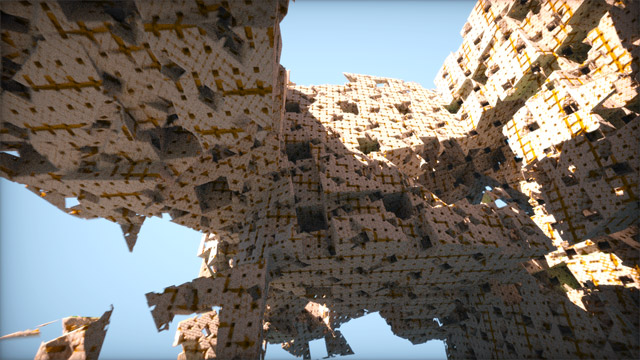
\includegraphics[scale=0.36]{images/cover}
}
\subtitle{}
\author[Dr. Johannes Riesterer] % (optional, for multiple authors)
{Dr.  rer. nat. Johannes Riesterer}

\date[KPT 2004] % (optional)
{}

\subject{Computergrafik}


\begin{frame}
    \frametitle{Computergrafik}
\framesubtitle{}
    \begin{block}{Echzeit Darstellung}
\begin{table}[h]
    \centering
    \begin{tabular}{|l|l|}
    \hline
    \textbf{Echtzeit-Typ} & \textbf{Eigenschaften} \\ \hline
    \textbf{Harte Echtzeit} & \begin{tabular}[c]{@{}l@{}}Zeitlimits zwingend, \\ Systemfehler bei Verpassen.\end{tabular} \\ \hline
    \textbf{Weiche Echtzeit} & \begin{tabular}[c]{@{}l@{}}Kleine Abweichungen erlaubt, \\ Leistung sinkt bei Überschreitung.\end{tabular} \\ \hline
    \end{tabular}
   % \caption{Definitionen von Echtzeitsystemen}
    \end{table}
    
\end{block}

\end{frame}


\begin{frame}
    \frametitle{Computergrafik}
\framesubtitle{}
    \begin{block}{Echzeit Darstellung}
Standard: $60$ Frames pro Sekunde bei einer Bildschirmauflösung von $4K=3840 \times 2160$ Pixel.  
D.h. $497.664.000$ Farbwerte müssen pro Sekunde berechnet und an das Ausgebegerät
geschickt werden. 
Kombination von Soft- und Hardware nötig.
\end{block}
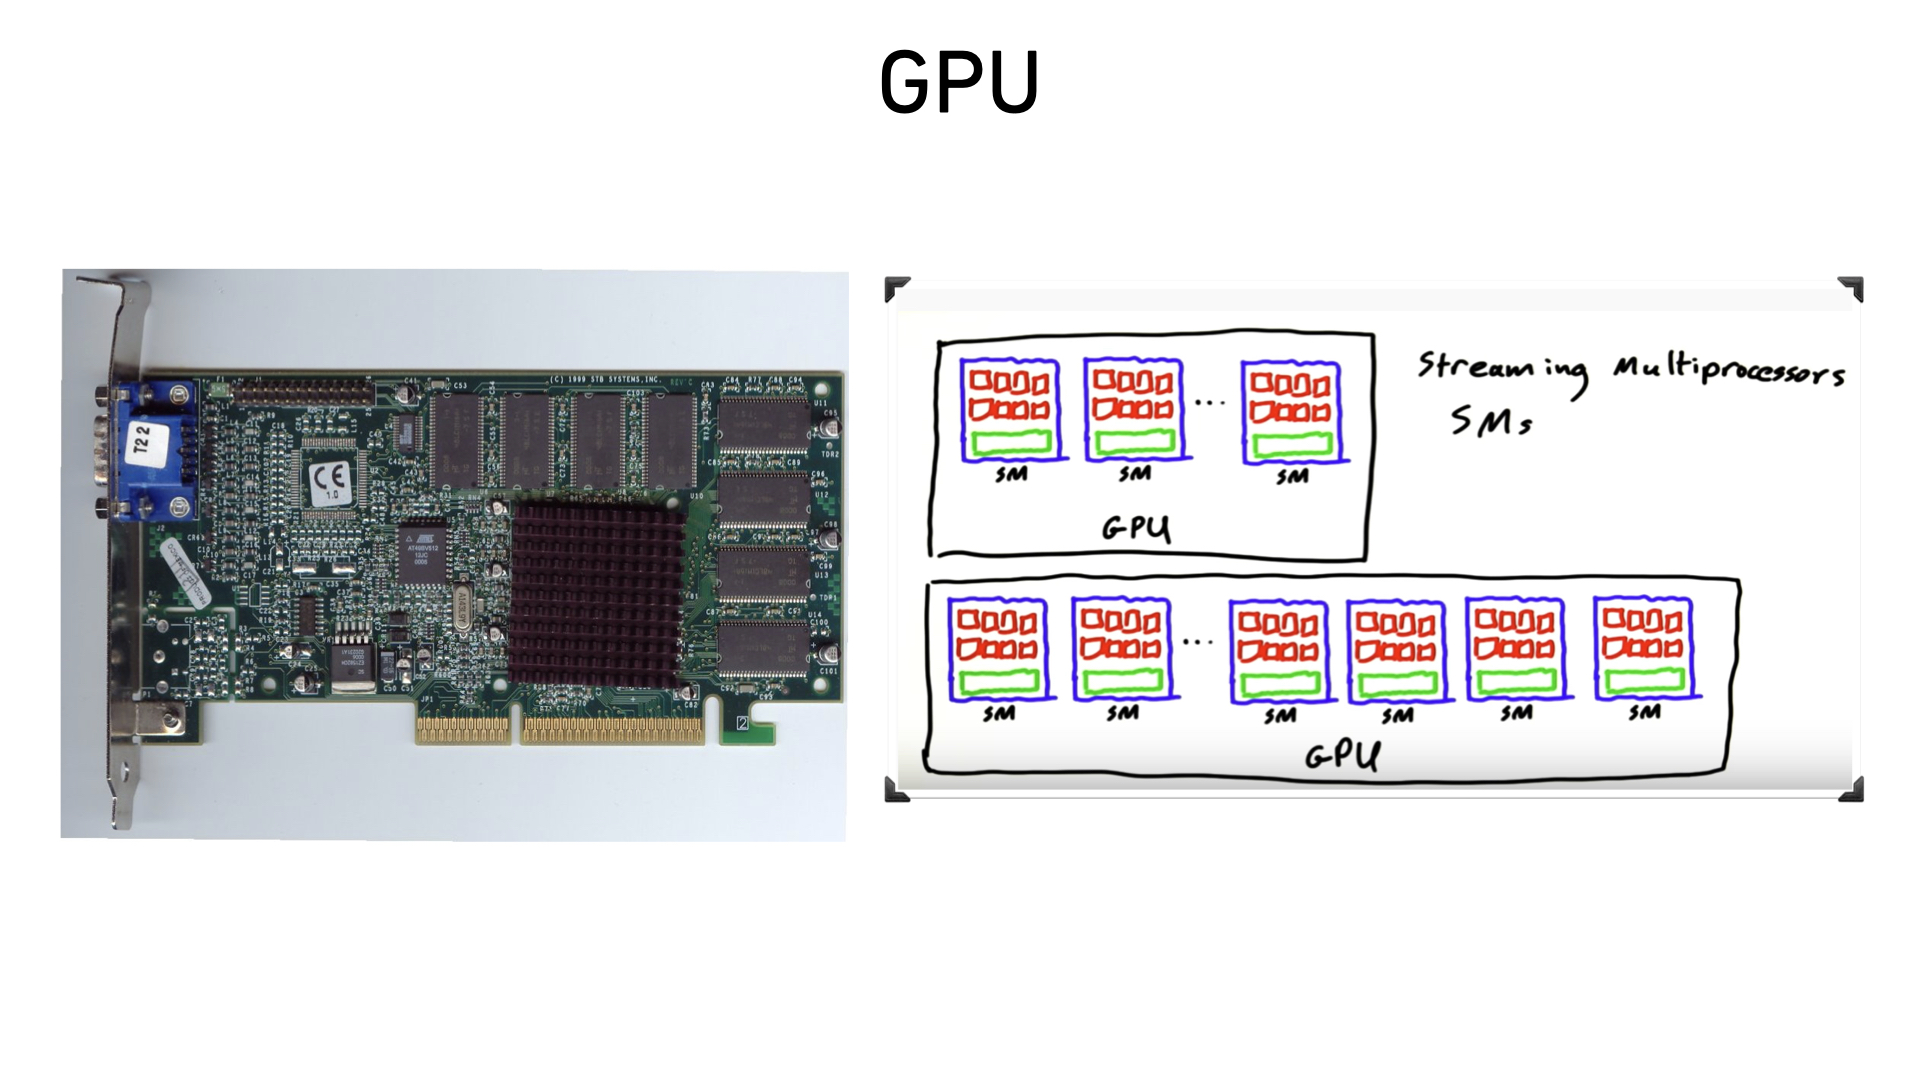
\includegraphics[scale=0.14]{images/Shaderday_Intro/Shaderday_Intro_004} \\

\end{frame}



\begin{frame}{Aufbau und Funktionsweise einer GPU}
    \begin{itemize}
      \item \textbf{Architektur:} Viele einfache Rechenkerne in \textit{Streaming Multiprocessors (SM)}, optimiert für parallele Berechnung.
      \item \textbf{Speicherhierarchie:}
      \begin{itemize}
        \item \textit{Global Memory (VRAM)}: Großer, langsamer Speicher für die gesamte GPU.
        \item \textit{Shared Memory}: Schneller Zwischenspeicher pro SM.
        \item \textit{Register}: Klein, extrem schnell, lokal pro Kern.
      \end{itemize}
      \item \textbf{SIMD-Prinzip:} Gleiche Operation auf mehrere Daten gleichzeitig (Single Instruction, Multiple Data).
      \item \textbf{Thread-Modell:} Threads in \textit{Thread-Blocks} organisiert, diese in einem \textit{Grid}.
      \item \textbf{Spezialisierte Hardware:} Rasterisierung, Texturierung und Shading für Grafikoperationen.
    \end{itemize}
  \end{frame}



\begin{frame}
    \frametitle{Computergrafik}
\framesubtitle{}

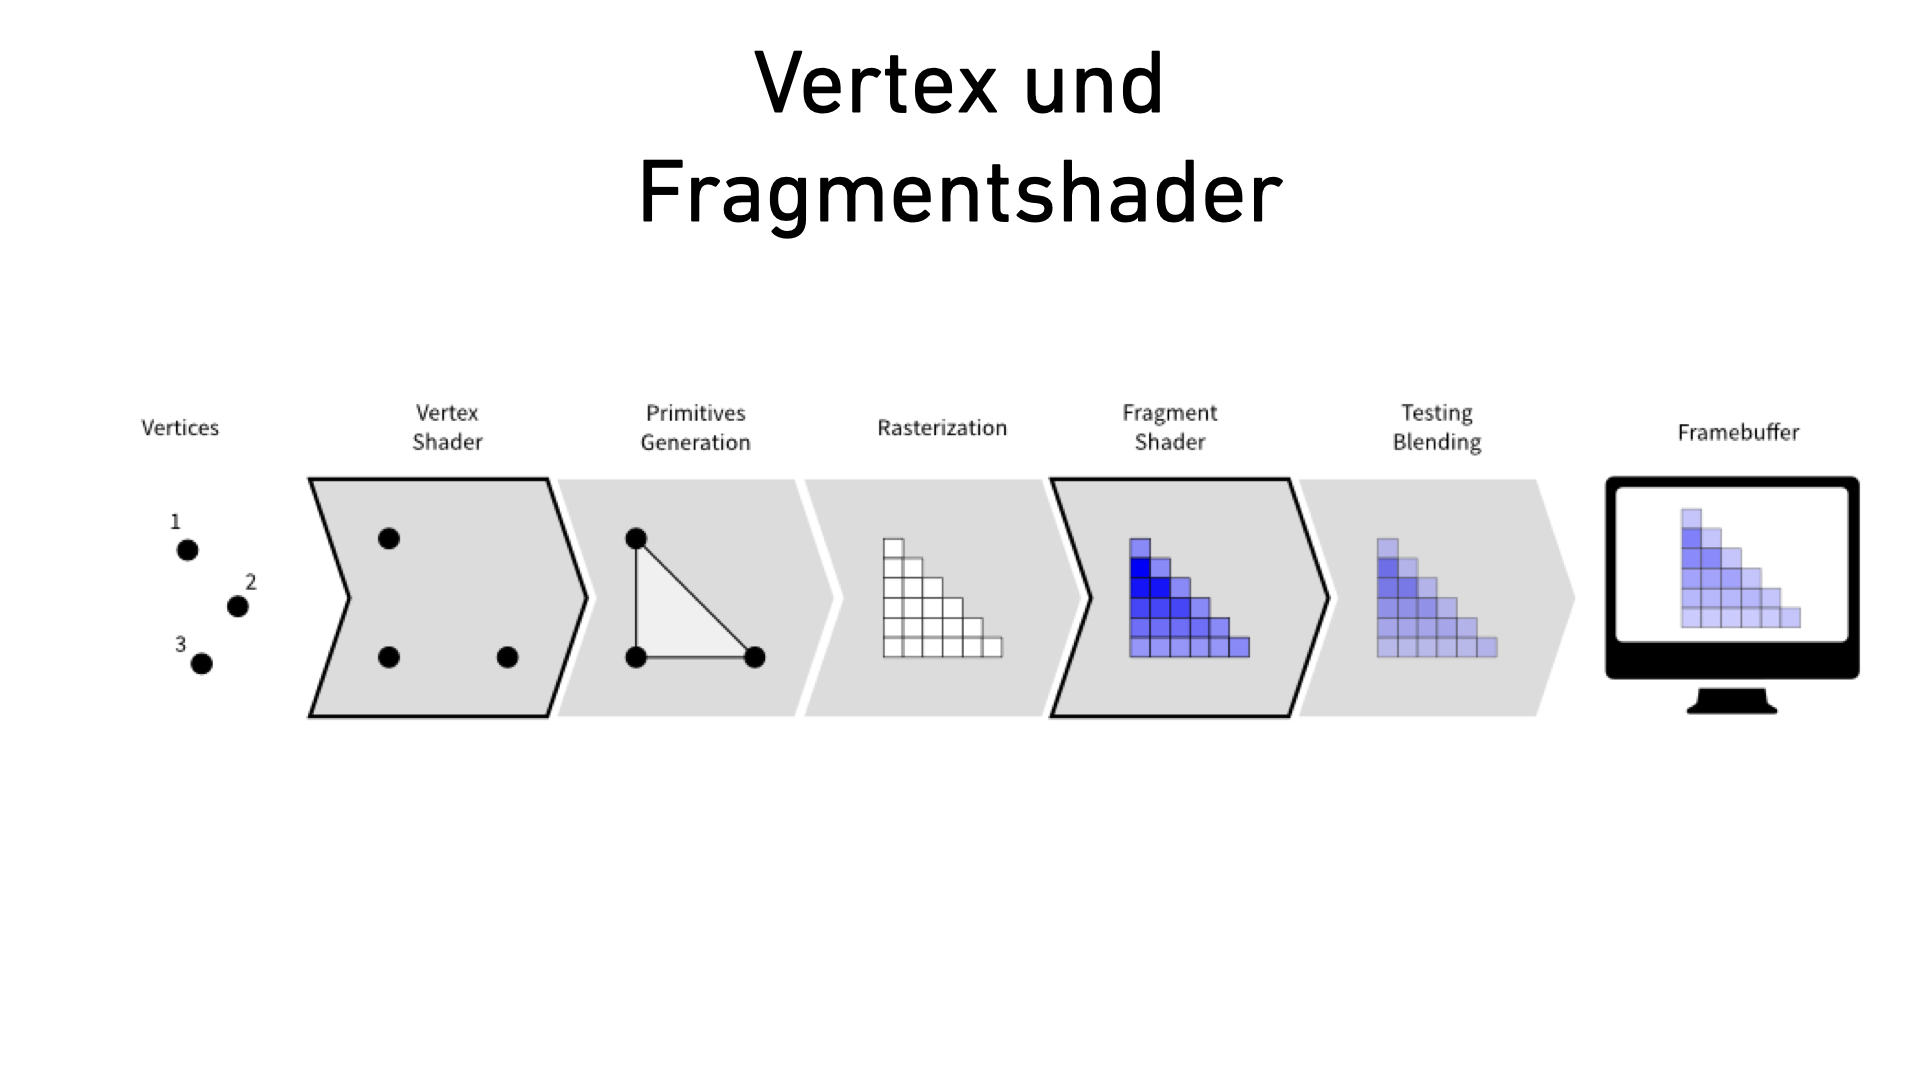
\includegraphics[scale=0.15]{images/Shaderday_Intro/Shaderday_Intro_007}

\end{frame}


\begin{frame}
    \frametitle{Computergrafik}
\framesubtitle{}

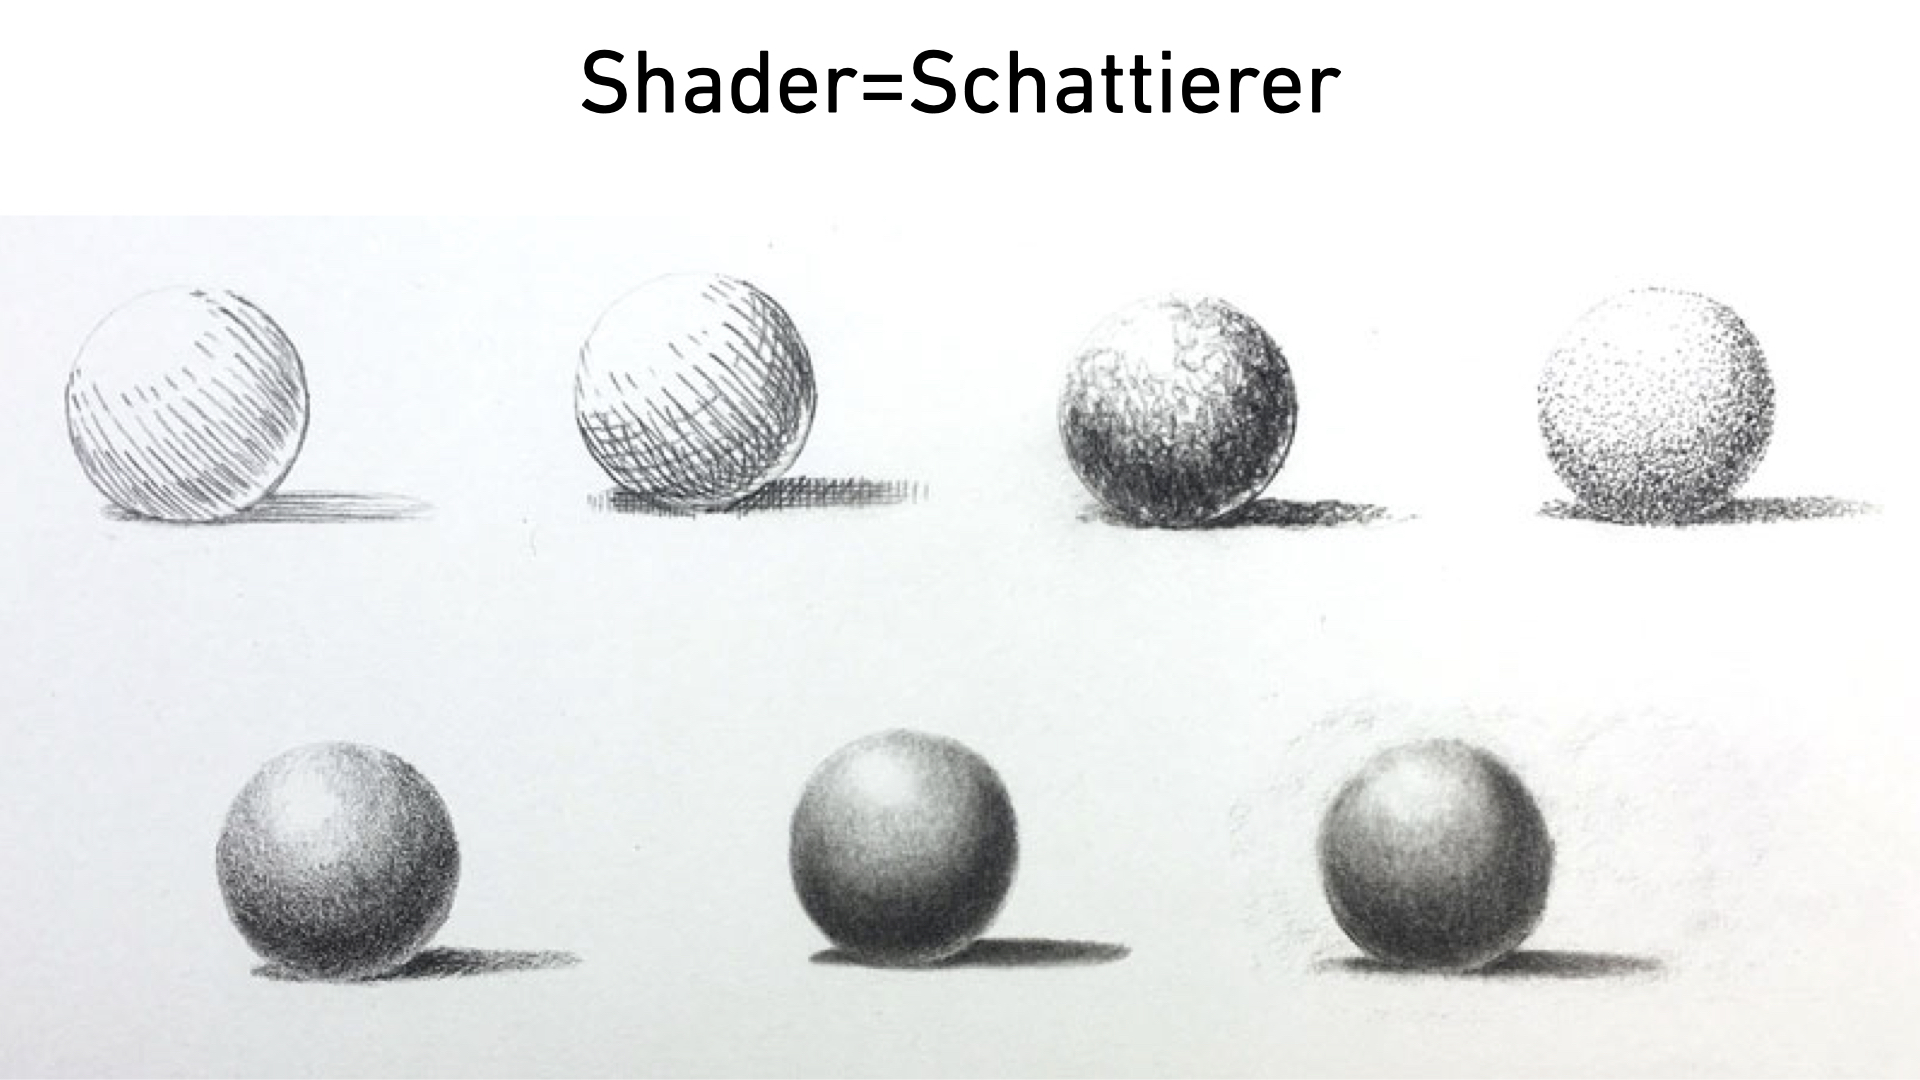
\includegraphics[scale=0.15]{images/Shaderday_Intro/Shaderday_Intro_001} 
\end{frame}



  
\begin{frame}
    \frametitle{ Shaderprogramm}
\framesubtitle{}
\begin{center}
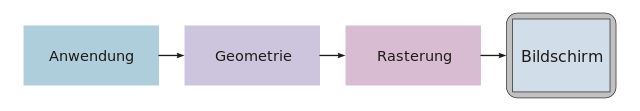
\includegraphics[scale=0.26]{images/cgpipeline_grob}
\\
\includegraphics[scale=0.20]{images/Zeichnung_Shaderpipeline}

\end{center}
\end{frame}

\begin{frame}
    \frametitle{OpenGL Pipeline}
\framesubtitle{}
    \begin{block}{}
\begin{center}
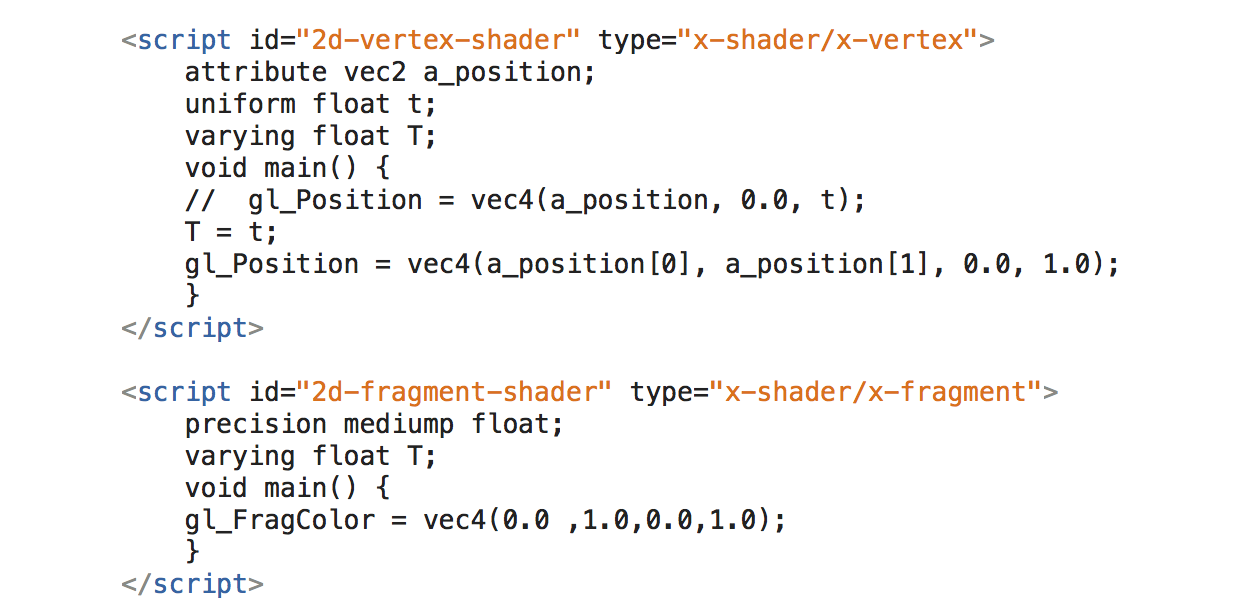
\includegraphics[scale=0.56]{images/shader}
\end{center}
\end{block}
\end{frame}



\end{document}
